\documentclass[11pt,a4paper]{article}
\usepackage[T1]{fontenc}
\usepackage[margin=2.3cm]{geometry}
\usepackage{amsmath,amssymb}
\usepackage{graphicx}
\usepackage[dvipsnames]{xcolor}
\usepackage{enumitem}
\usepackage[colorlinks=true,linkcolor=blue,urlcolor=blue]{hyperref}
\setlength{\parskip}{0.6em}
\setlength{\parindent}{0pt}
\begin{document}

\begin{center}{\LARGE\bfseries opensymbolic}\\[0.4em]{\large Let a computer rediscover a physical law from data, in three sessions.}\\[0.2em]\small PAN IIT OSS explainer \textbullet{} higher secondary to advanced undergraduate (levels 4-6)\end{center}

\section*{Why this exists}
Instead of fitting a flexible curve and trusting it, symbolic regression searches for a formula and balances accuracy against simplicity. This explainer shows how a formula becomes a tree, how complexity and error trade off, and how a small search can rediscover a physical law.

\section*{The end goal}
Rediscover physical laws with symbolic regression. The end goal is to rediscover physical laws with symbolic regression, the same idea researchers use to look for interpretable rate rules in combustion chemistry, where a rule written as a formula can be checked against known physics.

\section*{How the three sessions build up}
\begin{enumerate}[nosep]
\item \textbf{Session 1: Data that follow a law: can a computer guess the formula?} (Level 1, conceptual interactive model, 60 min).
\item \textbf{Session 2: A formula is a tree: simple versus accurate} (Level 2, mathematical engineering model, 75 min).
\item \textbf{Session 3: A real formula search: recover the law, measure the success rate} (Level 3, simulation and validation, 90 min).
\end{enumerate}

\section{Session 1: Data that follow a law: can a computer guess the formula?}

\subsection*{A. Real-world problem}
Drop a ball from a tower and time how far it has fallen after each half second. The numbers rise faster and faster, but is the distance proportional to the time, to its square, to its cube? Galileo had to guess a formula and test it. A computer can do the guessing: write many candidate formulas, fit each one, and keep the one that matches the data best. That is the seed of symbolic regression, a method that finds an equation rather than only a curve, and that scientists use today to look for interpretable rules in chemistry, for example for reaction rates.

\subsection*{B. Concept and theory}
Free fall from rest follows d = (1/2) g t\textasciicircum{}2, where d is the distance fallen in metres, t the time in seconds and g the acceleration due to gravity, 9.81 m/s\textasciicircum{}2 on Earth. Real measurements carry errors, so we model them by multiplying each distance by (1 + e) with a small fractional error e. A candidate formula has the form d = c t\textasciicircum{}n: the exponent n is chosen by the search and the constant c is found by least squares. Minimising the sum of squared differences between data and formula gives c = sum(f d) / sum(f f), where f = t\textasciicircum{}n. The score is the mean squared error (MSE): the average of the squared differences, in metres squared. If the winning exponent is 2, then c = g / 2 and so g = 2c.

\begin{itemize}[nosep]
\item d: distance fallen from rest (m)
\item t: time since release (s)
\item g: acceleration due to gravity (m/s\textasciicircum{}2)
\item c: the constant fitted for a candidate formula (m/s\textasciicircum{}n)
\item n: exponent of t in the candidate (no unit)
\item MSE: mean squared error of a candidate (m\textasciicircum{}2)
\item e: fractional measurement error of one point (no unit)
\end{itemize}

\begin{equation*}
d=\tfrac12\,g\,t^2
\end{equation*}

\begin{equation*}
c=\frac{\sum_i f_i\,d_i}{\sum_i f_i^2},\qquad f_i=t_i^{\,n}
\end{equation*}

\begin{equation*}
\mathrm{MSE}=\frac1N\sum_{i=1}^{N}\big(d_i-c\,t_i^{\,n}\big)^2
\end{equation*}

\begin{equation*}
d=c\,t^2\ \Rightarrow\ g=2c
\end{equation*}

\begin{center}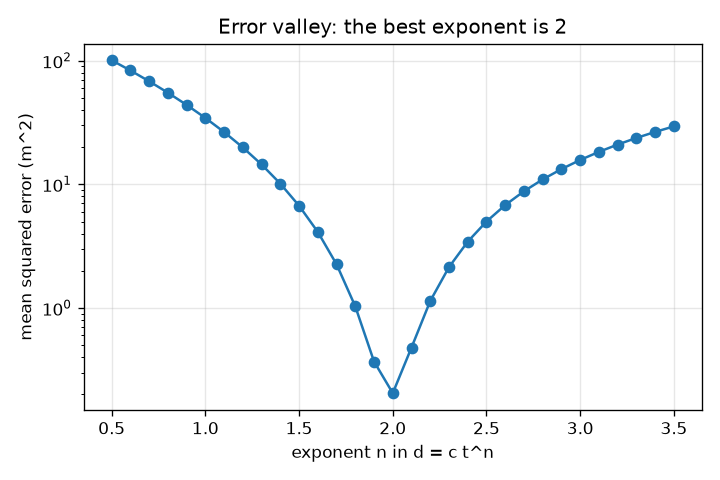
\includegraphics[width=0.85\linewidth]{figures/s01_error_vs_exponent.png}\\\small Error against the exponent n: the valley is at n = 2.\end{center}

\subsection*{E. Worked example}
Fit d = c t\textasciicircum{}2 to the six measured distances for the falling ball (times 0.5, 1, 1.5, 2, 2.5, 3 s) and estimate g.
\begin{enumerate}[nosep]
\item Measured distances are 1.251, 4.758, 11.147, 19.228, 31.576 and 43.704 m (the true values times (1 + e)).
\item The shapes f = t\textasciicircum{}2 are 0.25, 1, 2.25, 4, 6.25 and 9. Their squares sum to sum(f f) = 142.1875.
\item Multiply each shape by its distance and add: sum(f d) = 697.742.
\item c = 697.742 / 142.1875 = 4.907 m/s\textasciicircum{}2.
\item The mean squared error is 0.205 m\textasciicircum{}2, and g = 2c = 9.81 m/s\textasciicircum{}2, the known value.
\end{enumerate}
\textbf{Answer.} c = 4.907, MSE = 0.205 m\textasciicircum{}2 and g = 9.81 m/s\textasciicircum{}2.

\subsection*{F. Questions}
\begin{enumerate}[nosep]
\item \textbf{Conceptual.} Two exponents, n = 1.9 and n = 2.1, give errors of 0.37 and 0.48 m\textasciicircum{}2, close to the 0.20 m\textasciicircum{}2 of n = 2. Can the data prove that n is exactly 2?
\item \textbf{Numerical.} A shape f = (1, 2) is fitted to the data d = (3, 5) with d = c f. Find c and the MSE by hand.
\item \textbf{Graph and simulation interpretation.} On the error-versus-exponent curve, the error at n = 1 is 34.39 m\textasciicircum{}2 and at n = 3 it is 15.73 m\textasciicircum{}2. Which wrong guess is worse, and where is the minimum?
\item \textbf{Design and optimisation challenge.} Design: you can time only four drops with a stopwatch accurate to about 0.1 s. Choose the drop times (or heights) and say how you would decide between n = 1.5, 2 and 3, and what would make your decision more reliable.
\end{enumerate}

\section{Session 2: A formula is a tree: simple versus accurate}

\subsection*{A. Real-world problem}
Kepler's third law links the time a planet needs to circle the Sun (its period T) to its distance a from the Sun. With six planets you can write a short formula, a medium one and a very flexible one, and all of them may fit the planets you used. Which would you trust to predict a planet farther out? A symbolic regression program faces this choice for millions of formulas, so it needs a way to measure how complicated a formula is and a way to test it on data it has not seen.

\subsection*{B. Concept and theory}
We store a formula as a tree. Leaves are the variable x or a number; inner nodes are operations: add, sub, mul, div (two children) and sqrt, exp, log, sq (one child). The complexity of the formula is the number of nodes. The error is the mean squared error on data. A formula is on the Pareto front if no other formula is both simpler (or equal) and more accurate. Flexible formulas can always lower the training error, so the training error alone favours the biggest formula; to judge honestly we hold out part of the data, never use it for fitting, and compare errors on it. Kepler's law is T\textasciicircum{}2 proportional to a\textasciicircum{}3, which means T = c a\textasciicircum{}(3/2) with c = 1 when T is in years and a in AU (astronomical units, the Earth-Sun distance).

\begin{itemize}[nosep]
\item a: semi-major axis of the orbit (AU)
\item T: orbital period (years)
\item c, c0..c3: constants fitted by least squares (depends on the formula)
\item nodes: complexity: number of nodes in the tree (no unit)
\item MSE: mean squared error (years\textasciicircum{}2)
\end{itemize}

\begin{equation*}
T^2\propto a^3\ \Rightarrow\ T=c\,a^{3/2}
\end{equation*}

\begin{equation*}
\text{complexity}=\text{number of nodes in the tree}
\end{equation*}

\begin{equation*}
\mathrm{MSE}=\frac1N\sum_i\big(f(a_i)-T_i\big)^2
\end{equation*}

\begin{equation*}
f_C(a)=c_0+a\big(c_1+a(c_2+c_3 a)\big)
\end{equation*}

\begin{center}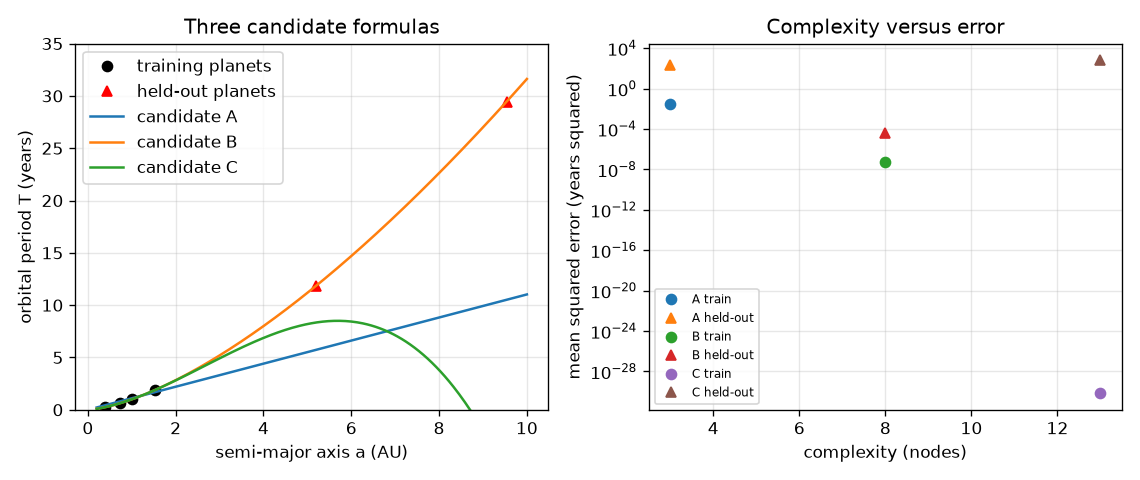
\includegraphics[width=0.85\linewidth]{figures/s02_kepler_candidates.png}\\\small Three candidate formulas on the planets, and their complexity versus error.\end{center}

\subsection*{E. Worked example}
Build the tree for T = c sqrt(a a a) with c = 1 and use it to predict the period of Mars (a = 1.524 AU). Count its complexity.
\begin{enumerate}[nosep]
\item The tree is mul(c, sqrt(mul(a, mul(a, a)))). Its nodes are mul, c, sqrt, mul, a, mul, a, a: 8 nodes (with c = 1 as a number node).
\item Evaluate from the leaves: a * a * a = 1.524\textasciicircum{}3 = 3.540.
\item Take the square root: sqrt(3.540) = 1.8814, and multiply by c = 1.
\item The observed period of Mars is 1.881 years, so the prediction matches to 3 decimals.
\item With the fitted constant (0.9999) the same tree predicts 11.867 years for Jupiter against an observed 11.862.
\end{enumerate}
\textbf{Answer.} Complexity 8 nodes; Mars: 1.8814 years against 1.881 observed.

\subsection*{F. Questions}
\begin{enumerate}[nosep]
\item \textbf{Conceptual.} Why is it not enough to choose the formula with the smallest training error?
\item \textbf{Numerical.} Draw the tree for x\textasciicircum{}2 - 2 using sq, sub and a number node. Count the nodes and evaluate it at x = 3.
\item \textbf{Graph and simulation interpretation.} On the complexity-versus-error plot, which candidate has the lowest training error and which the lowest held-out error? What does that tell you?
\item \textbf{Design and optimisation challenge.} Design: use the rule 'accept a formula only if its held-out error is below 0.01 years squared, and then choose the one with the fewest nodes'. Which candidate is chosen? What changes if Jupiter is moved into the training set?
\end{enumerate}

\section{Session 3: A real formula search: recover the law, measure the success rate}

\subsection*{A. Real-world problem}
You have measurements of a pendulum, a gas reaction or a falling body, and no formula. Can a program write the formula for you, and can you trust it? Real symbolic regression tools search over millions of formulas; here you build a small honest version, run it on synthetic data whose true law you know, and count how often it finds that law. You will also see how it can fail, and why physicists check units before they believe a formula.

\subsection*{B. Concept and theory}
The search enumerates all expression trees up to 7 nodes built from the variable x, the number 1 and the operations add, sub, mul, div, sqrt, sq, exp and log. Two trees that give the same numbers on the data are duplicates; the smaller is kept, and formulas giving nan or infinity are dropped. Each formula f is used as y = a f(x) + b: this is linear in a and b, so the best constants are exact: a = cov(f, y) / var(f) and b = mean(y) - a mean(f). The best formula at each size, kept only if it beats every smaller formula, forms the Pareto front. To choose from the front we minimise a score that rewards low error and punishes size: score = N ln(MSE) + (nodes + 2) ln N, where N is the number of data points and the +2 counts a and b (this is the Bayesian information criterion, BIC). Taking logarithms can turn a nonlinear constant into a linear one: for the Arrhenius law k = A exp(-E / T), ln k = ln A - E x / 1000 with x = 1000 / T, which is a straight line with slope -E / 1000 and intercept ln A. For power laws T = C L\textasciicircum{}p g\textasciicircum{}q m\textasciicircum{}r the units must match: the exponents must make kilograms, metres and seconds agree with those of the quantity on the left.

\begin{itemize}[nosep]
\item x, y: input and output of the data (depends on the law)
\item f: a candidate formula in x (depends)
\item a, b: scale and offset fitted exactly by least squares (units of y)
\item nodes: complexity of f (no unit)
\item N: number of data points (no unit)
\item T, E: temperature and activation temperature (E over the gas constant) (K)
\item p, q, r: exponents of L, g and m in a power law (no unit)
\end{itemize}

\begin{equation*}
y\approx a\,f(x)+b,\qquad a=\frac{\mathrm{cov}(f,y)}{\mathrm{var}(f)},\quad b=\bar y-a\bar f
\end{equation*}

\begin{equation*}
\mathrm{score}=N\ln\mathrm{MSE}+(\text{nodes}+2)\ln N
\end{equation*}

\begin{equation*}
\ln k=\ln A-\frac{E}{1000}\,x,\qquad x=\frac{1000}{T}
\end{equation*}

\begin{equation*}
T=C\,L^p g^q m^r:\quad [\mathrm{kg}]:\ r=0,\ \ [\mathrm{m}]:\ p+q=0,\ \ [\mathrm{s}]:\ -2q=1
\end{equation*}

\begin{center}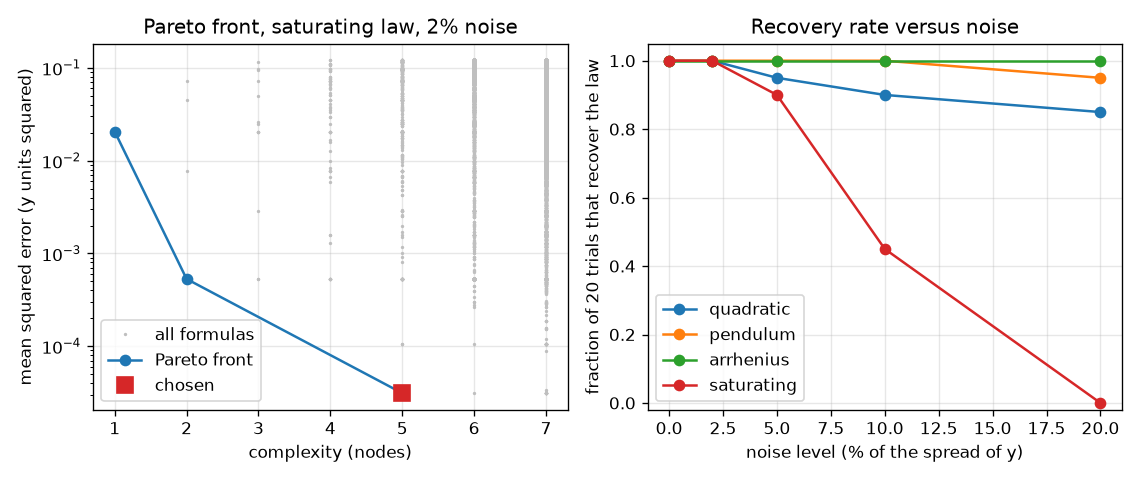
\includegraphics[width=0.85\linewidth]{figures/s03_search_front.png}\\\small Left: the Pareto front for the saturating law at 2 percent noise. Right: recovery rate versus noise for the four laws.\end{center}

\subsection*{E. Worked example}
Run the search on noise-free data from y = 3 x\textasciicircum{}2 (30 points, x from 0.5 to 5). Which formula is chosen and with which constants?
\begin{enumerate}[nosep]
\item Enumeration up to 7 nodes on these x values keeps 11777 distinct formulas (518 up to 5 nodes).
\item For every formula the exact fit gives a, b and the error.
\item The Pareto front starts with x (a straight line fits poorly) and reaches the best error at sq(x), 2 nodes.
\item For sq(x) the exact fit returns a = 3.000 and b = 0.000 with an error at the level of round-off, so the search recovers y = 3 x\textasciicircum{}2.
\item Every larger formula at the noise-free error is a duplicate or a worse choice because of the size penalty.
\end{enumerate}
\textbf{Answer.} The chosen formula is sq(x) with a = 3.000 and b = 0.000: the law is recovered exactly.

\subsection*{F. Questions}
\begin{enumerate}[nosep]
\item \textbf{Conceptual.} Why does fitting y = a f(x) + b make the search much faster than trying many values of the constants one by one?
\item \textbf{Numerical.} Fit y = a f + b by hand to the data y = (1, 3, 5) at f = (0, 1, 2). Give a, b and the error.
\item \textbf{Graph and simulation interpretation.} In the recovery-rate plot at 5 percent noise the rates for 40 trials are 97.5 percent for the quadratic, pendulum and Arrhenius laws and 87.5 percent for the saturating law; at 20 percent noise they are 87.5, 92.5, 97.5 and 0 percent. Interpret the difference.
\item \textbf{Design and optimisation challenge.} Design: a pendulum experiment used lengths L = g/2 by accident (so L and g are tied together), with the mass varied freely. Out of 729 exponent triples (p, q, r) from -2 to 2 in steps of 0.5, 9 fit equally well. How can units pick the right one, and how would you redesign the experiment so that fewer triples tie?
\end{enumerate}

\section{Real-world mini-project}
\textbf{Find a rate law from synthetic kinetics data.} A chemist measures the rate r = k c\textasciicircum{}n of a reaction at concentrations c from 0.2 to 2.0 mol/L; the true law has k = 0.5 and order n = 2, and every rate carries 5 percent noise (relative to the spread of the rates). Use \texttt{kinetics\_trial(n\_points, seed)} from Session 3, which runs the enumeration search on one noisy data set, and ask: how many concentration points must the chemist measure before the search recovers the order in at least 90 percent of repeated experiments? Then use the Arrhenius law from Session 3 (ln k against 1000 / T) to recover the activation temperature E from noisy rate constants.

\section{The path ahead}
\begin{enumerate}[nosep]
\item \textbf{Session 4: Constants inside the formula.} A search that fits two constants inside the formula by iteration, not only a and b outside.
\item \textbf{Session 5: More than one input.} A search over formulas in x1 and x2 that recovers r = x1 sqrt(x2).
\item \textbf{Session 6: Weighted errors.} A weighted least-squares version of the search.
\item \textbf{Session 7: A genetic search for bigger spaces.} A genetic loop with a complexity penalty.
\item \textbf{Session 8: Leave-one-class-out validation.} A validation function that holds out one class of synthetic reactions at a time.
\end{enumerate}

\section{Answers and hints}

\subsection*{Session 1}
\begin{enumerate}[nosep]
\item \textbf{Conceptual.} Hint: Think about the measurement errors of up to 3 percent. Solution: No. The data show that n is close to 2 and that n = 1 or n = 3 are far worse, but with errors of a few percent the neighbouring exponents 1.9 and 2.1 are only about twice as bad. A law is chosen because it is the simplest formula that fits within the noise and also has a physical reason (here d = (1/2) g t\textasciicircum{}2 from constant acceleration), not because the error is exactly zero.
\item \textbf{Numerical.} Hint: Use c = sum(f d) / sum(f f), then average the squared differences. Solution: sum(f d) = 1*3 + 2*5 = 13 and sum(f f) = 1 + 4 = 5, so c = 13/5 = 2.6. The formula gives (2.6, 5.2), so the differences are 0.4 and -0.2 and MSE = (0.16 + 0.04) / 2 = 0.1. Units: the square of the units of d.
\item \textbf{Graph and simulation interpretation.} Hint: Compare the heights of the curve at n = 1 and n = 3 and find the lowest point. Solution: The minimum is at n = 2.0 with error 0.20 m\textasciicircum{}2. The exponent 1 is worse than the exponent 3 here (34.39 against 15.73 m\textasciicircum{}2). The valley is not symmetric because the times lie between 0.5 and 3 s, and a t\textasciicircum{}3 curve is closer to t\textasciicircum{}2 over that range than a straight line is.
\item \textbf{Design and optimisation challenge.} Hint: Spread the times widely and repeat measurements; remember that the distance error depends on the timing error. Solution: Use times spread over the whole range, for example 0.5 to 3 s, because the candidates only differ clearly at large t. Repeat each drop several times and average to reduce the timing error. Fit every candidate and compare MSE; prefer the simplest candidate within the noise. A further constraint is that long drops need a tall tower and air drag grows with speed. The trade-off is range (more distinguishing power) against practicality and drag.
\end{enumerate}

\subsection*{Session 2}
\begin{enumerate}[nosep]
\item \textbf{Conceptual.} Hint: Think about a formula with as many constants as data points. Solution: A flexible formula can pass exactly through the training points, so its training error can reach almost zero (the cubic here has an error below 1e-20 on four points), while its predictions elsewhere are wild (held-out error 645.0 years squared). The training error rewards flexibility, not truth. We need a held-out set or a penalty for complexity.
\item \textbf{Numerical.} Hint: The root is the subtraction. Its children are sq(x) and the number 2. Solution: The tree is sub(sq(x), 2): nodes sub, sq, x, 2, so complexity 4. At x = 3: sq(3) = 9 and 9 - 2 = 7.
\item \textbf{Graph and simulation interpretation.} Hint: Compare the three markers for training and held-out error. Solution: C (13 nodes) has the lowest training error but the highest held-out error (645.0 years squared). B (8 nodes) has a held-out error of about 4e-5 years squared, far better than A (198.2) and C. So training error and trustworthiness are different things; the held-out error picks B.
\item \textbf{Design and optimisation challenge.} Hint: Compute the held-out errors of A, B and C. For the second part train on five planets and hold out only Saturn. Solution: Only B passes the threshold (A: 198.2, C: 645.0), so B is chosen. With five training planets (Mercury to Jupiter) and Saturn held out, C's held-out error is still 43.4 years squared, B's is below 1e-3, so B is still chosen. Trade-off: more training data helps the flexible formula but not enough; a formula with the right structure needs fewer data.
\end{enumerate}

\subsection*{Session 3}
\begin{enumerate}[nosep]
\item \textbf{Conceptual.} Hint: What kind of problem is least squares when a and b enter linearly? Solution: When the constants enter linearly there is an exact formula for the best a and b, so every formula is fitted in one step without iteration, and we can fit thousands of formulas with one matrix operation. Constants inside the formula (like E in exp(-E x)) need an iterative nonlinear search; this is why we took the log of the Arrhenius law.
\item \textbf{Numerical.} Hint: The data are exactly on a straight line in f. Solution: The mean of f is 1 and the mean of y is 3. cov = ((-1)(-2) + 0*0 + 1*2)/3 = 4/3 and var(f) = (1 + 0 + 1)/3 = 2/3, so a = 2. Then b = 3 - 2*1 = 1. The formula 2 f + 1 reproduces the data exactly, so the error is 0.
\item \textbf{Graph and simulation interpretation.} Hint: Which law has the formula with the most nodes, and what does noise do to the front? Solution: The saturating law y = 2x/(1+x) needs 5 nodes and its curve is smooth and close to simpler formulas, so noise lets simpler wrong formulas win the penalised score; at 20 percent noise it is never recovered. The Arrhenius law becomes a straight line in the log form, so the simplest formula x is the true one and noise cannot hide it. Rates below 100 percent at low noise also show that the criterion sometimes picks a wrong formula by chance.
\item \textbf{Design and optimisation challenge.} Hint: Write the dimension of L\textasciicircum{}p g\textasciicircum{}q m\textasciicircum{}r in kilograms, metres and seconds and compare with a time. Solution: A time needs the exponent of kg to be 0 (r = 0), of metres 0 (p + q = 0) and of seconds 1 (-2q = 1), so q = -0.5 and p = 0.5. Only one of the 729 triples passes, and its constant is C = 6.17, within 2 percent of 2 pi = 6.283. To get fewer ties the experimenter should vary L and g independently so that their effects are separable. Trade-off: units remove impossible formulas but cannot fix a poorly designed experiment, and they say nothing about dimensionless constants such as 2 pi.
\end{enumerate}

\section{How to join}
Read \texttt{CONTRIBUTING.md} in the repository, then pick an issue labelled \texttt{good first issue}. Repository: \url{https://github.com/KrunalPanchal1995/opensymbolic}

\end{document}
